\documentclass[letterpaper]{l3doc}

\usepackage[mono = false]{libertine}
\usepackage{geometry,pdfpages,tikz,tabularx,xfrac,hologo,authblk}
\hologoFontSetup{general = \sffamily}
\newenvironment{example}{\begin{list}{}{\leftmargin=3em}\item }{\end{list}}
\fvset{xleftmargin = \parindent}
\usepackage[fontset = none]{ctex}
\setCJKmainfont[AutoFakeBold = 4, AutoFakeSlant]{LXGW WenKai}
\setCJKsansfont[AutoFakeBold = 4, AutoFakeSlant]{LXGW WenKai}
\setCJKmonofont[AutoFakeBold = 4, AutoFakeSlant]{LXGW WenKai}
\usepackage[os = mac]{menukeys}

\title{
    \cls{litetable} 文檔類:多彩嘅課程表
    \thanks{\url{https://github.com/xiamyphys/litetable}}
}

\author{夏明宇,杭州電子科技大學}

\affil{\href{mailto:xiamyphys@gmail.com}{xiamyphys@gmail.com}}

\date{Version 3.0B, \today}

\begin{document}

\maketitle

\begin{abstract}
    本文檔系 \cls{litetable} 文檔類嘅用户手冊放. 應該文檔類提供咗個多彩嘅課程表設計. 歡迎通過郵件 \href{mailto:xiamyphys@gmail.com}{xiamyphys@gmail.com} 或者 \href{https://github.com/xiamyphys/litetable/issues}{GitHub} 建議或者反饋bug. 本手冊提供英語、中文和\textbf{粵語}版本.
\end{abstract}

\section{介紹}

\subsection{所使宏包}

應該文檔類基於 \cls{article} 文檔類. 要 \pkg{expl3},\pkg{xparse},\pkg{tikz},\pkg{listofitems} 同 \pkg{xcolor} 宏包. 

\subsection{相容性}

所使 \pkg{expl3} 宏包嘅版本使支持``e-type''變體,所以要文檔類唔可以喺 \hologo{TeX}Live 2023 同更早嘅版本上運行. 所用嘅測試平台為 macOS 15.1 / Overleaf / Ubuntu 22.04.2,並使用 \hologo{TeX}Live 2024 發行版,喺 \hologo{pdfLaTeX} 同 \hologo{XeLaTeX} 編譯器下均可正常運行. Windows 同 Unix 平台嘅相容性未知.

\section{使用}

\subsection{載入 \cls{litetable} 並建置課程表框架}

同載入其他文檔類一樣,只令寫下

\begin{Verbatim}
    \documentclass{litetable}
\end{Verbatim}

跟住落嚟嘅命令需要帶有 \cmd{remember picture,overaly} 選項嘅 \cmd{tikzpicture} 環境.

\subsubsection{命令:\cs{maketable}}

\begin{example}
    \cs{maketable}\oarg{semester}\marg{title}
\end{example}

此命令有兩個參數,可建置一個空白嘅課程表框架. 第一個可選參數可喺頁面嘅嘅右度角添加學期塊,第二個強制參數可指定標題.

\subsubsection{命令:\cs{more}}

\begin{example}
    \cs{more}\marg{comment}
\end{example}

此命令可喺頁面嘅嘅右下角添加備注.

\subsubsection{命令:\cs{timelist}}

\begin{example}
    \cs{timelist}\oarg{rows}\marg{time list}
\end{example}

此命令有兩個參數,第一個可選參數可直接決定課程表嘅行數,第二個強制參數可喺課程表嘅左側添加時間表. 輸入表格式如下:開始時間同結束時間之間用短線 (-) 分隔,並用逗號 (,) 系咪喺時間組之間分隔. 例如

\begin{Verbatim}
    \timelist[13]{%
        08:05 - 08:50, 08:55 - 09:40, 10:00 - 10:45, 10:50 - 11:35,
        11:40 - 12:25, 13:30 - 14:15, 14:20 - 15:05, 15:15 - 16:00,
        16:05 - 16:50, 18:30 - 19:15, 19:20 - 20:05, 20:10 - 20:55,
    }
\end{Verbatim}

對於兩個參數唔同使用情況,\cls{litetable} 會以如下規則建置對應行數嘅課程表框架.

\begin{table}[htbp]
    \centering
    \begin{tabularx}{.9\textwidth}{c X X}
      \toprule
        $\displaystyle\sfrac{\oarg{\#1}}{\marg{\#2}}$ &
        \multicolumn{1}{c}{使用} &
        \multicolumn{1}{c}{唔使用}\\
      \midrule
        使用 &
        效果與 \marg{\#2} 所描述嘅相同,但課程表嘅行數由 \oarg{\#1} 決定 &
        效果與 \oarg{\#1} 所描述嘅相同\\
      \midrule
        不使用 &
        效果與 \marg{\#2} 所描述嘅相同&
        ERROR!\\
      \bottomrule
    \end{tabularx}
\end{table}

\begin{itemize}
    \item 若強制參數 \marg{\#2} 接受咗$X$組時間,可選參數 \oarg{\#1} 接受嘅值為$X+a$,就課程表嘅左側得$1 \sim X$行會顯示時間,後面幾行唔顯示時間.
    \item 若強制參數 \marg{\#2} 接受咗$X+a$組時間,可選參數 \oarg{\#1} 接收嘅值為$X$, 就課程表嘅左側得$X$行嘅課程表,多餘嘅時間組將畀忽略,並返回一個警告.
\end{itemize}

\subsubsection{命令:\cs{weeklist}}

\begin{example}
    \cs{weeklist}\oarg{default weeks}\marg{week list}
\end{example}

此命令有兩個參數. 第一個可選參數可決定預設嘅星期數並會喺每課程塊嘅嘅右下角顯示,第二個強制參數可喺課程表嘅頂部添加對應寬度比例嘅工作日. 輸入表嘅第一行為工作日格式,第二行為對應嘅寬度比例,兩得之間用分號 (;) 分隔. 例如

\begin{Verbatim}
    \weeklist[Weeks 1 - 16]{%
        \scshape Mon,    \scshape Tue,     \scshape Wed,
        \scshape Thu,    \scshape Fri;     4,5,4,6,5
    }
\end{Verbatim}

\begin{figure}[!ht]
    \centering
    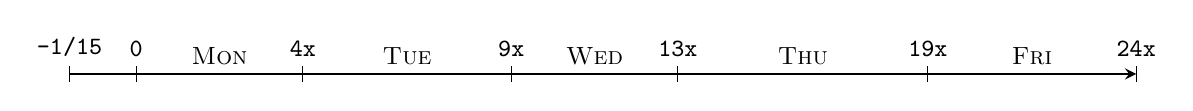
\begin{tikzpicture}[every node/.style={font=\small\sffamily\scshape}]
        \draw [thick,->,>=stealth] (-5 in/15,0) -- (5 in,0);
        \draw (-5 in/15,-.1) --++ (0,.2) node [above] {\verb|-1/15|};
        \draw (0,-.1) --++ (0,.2) node [above] {\verb|0|};
        \draw (4*5 in/24,-.1) --++ (0,.2) node [above] {\verb|4x|};
        \draw (9*5 in/24,-.1) --++ (0,.2) node [above] {\verb|9x|};
        \draw (13*5 in/24,-.1) --++ (0,.2) node [above] {\verb|13x|};
        \draw (19*5 in/24,-.1) --++ (0,.2) node [above] {\verb|19x|};
        \draw (5 in,-.1) --++ (0,.2) node [above] {\verb|24x|};
        \node [above] at (2*5 in/24,0) {Mon};
        \node [above] at (6.5*5 in/24,0) {Tue};
        \node [above] at (11*5 in/24,0) {Wed};
        \node [above] at (16*5 in/24,0) {Thu};
        \node [above] at (21.5*5 in/24,0) {Fri};
    \end{tikzpicture}
\end{figure}

此時 \cs{course} 命令中鍵 \keys{weeks} 嘅默認值畀賦為 \cmd{Weeks 1 - 16}. 如果輸入工作日嘅數量過輸入嘅寬度比例數量多,就多餘工作日將畀忽略並返回一條警告.

\subsection{添加課程塊}

使用 \cs{course} 命令喺當前工作日添加課程塊. 此命令有兩個參數.

\begin{example}
    \cs{course}\oarg{keyvals}\marg{class start number}\oarg{class end number}
\end{example}

第一個可選參數接受下列鍵:\keys{color} \keys{subject} \keys{location} \keys{teacher} \keys{weeks}. 鍵 \keys{color} 嘅默認值為 \cmd{DarkSlateGray},鍵 \keys{weeks} 嘅默認值由命令 \cs{weeklist} 嘅第一個參數決定. 第二個同第三個強制參數勒分別為課程嘅開始同結束序號. \cs{course} 命令嘅用例如下

\begin{Verbatim}
    \course [ color = DarkGreen, subject = listofitems, 
              location = French, teacher = Christian Tellechea
            ] {10} {12}
\end{Verbatim}

\begin{center}
    \noindent\fbox{
        \parbox{.96\linewidth}{
            將此課程塊嘅顏色設置為 \cmd{DarkGreen},此課程名為 \cmd{listofitems},上堂地方為 \cmd{French},老師為 \cmd{Christian Tellechea},喺當日嘅第 \cmd{10} 節課開始,第 \cmd{12} 節課結束.
        }
    }
\end{center}

\begin{itemize}
    \item 可通過 \cs{newday} 命令切換到落個工作日.
    \item 若課程塊嘅高度淨系得個單位,即$\marg{class start number} = \marg{class end number}$,就鍵 \keys{location} 同 \keys{teacher} 嘅值將輸出喺同一行並以逗號 (,) 隔,鍵 \cmd{weeks} 嘅值將唔會輸出.
    \item 若鍵 \keys{location} 同 \keys{teacher} 均未賦值,就鍵 \keys{subject} 嘅值將輸出喺課程塊嘅中心.
\end{itemize}

\includepdf[pages = 1]{litetable-demo.pdf}

\end{document}